\documentclass[UTF8,a4paper,fontset=fandol]{ctexart}

\usepackage[a4paper,top=2.2cm,bottom=2.2cm,left=2.2cm,right=2.2cm]{geometry}
\usepackage{amsmath,amssymb}
\usepackage{booktabs}
\usepackage{tabularx}
\usepackage{multirow}
\usepackage{graphicx}
\usepackage{xcolor}
\usepackage{tikz}
\usepackage{pgfplots}
\usepackage{subcaption}
\usepackage{caption}
\usepackage{float}
\usepackage{hyperref}

\usetikzlibrary{arrows.meta,positioning,shapes.geometric,fit,calc}
\pgfplotsset{compat=1.18}

\definecolor{journalblue}{HTML}{1F4E79}
\definecolor{journalteal}{HTML}{2A9D8F}
\definecolor{journalorange}{HTML}{E76F51}
\definecolor{journalyellow}{HTML}{E9C46A}
\definecolor{journalgray}{HTML}{64748B}
\definecolor{lightblue}{HTML}{EFF6FB}
\definecolor{lightteal}{HTML}{E9F7F5}
\definecolor{lightorange}{HTML}{FCEDE9}

\hypersetup{
  colorlinks=true,
  linkcolor=journalblue,
  citecolor=journalblue,
  urlcolor=journalblue
}

\setlength{\parindent}{2em}
\setlength{\parskip}{0pt}
\linespread{1.05}
\captionsetup{font=small,labelfont=bf,labelsep=quad}
\renewcommand{\figurename}{图}
\renewcommand{\tablename}{表}
\renewcommand{\refname}{参考文献}

\ctexset{
  section={
    format=\large\bfseries\color{journalblue},
    beforeskip=0.75em,
    afterskip=0.35em
  },
  subsection={
    format=\normalsize\bfseries,
    beforeskip=0.55em,
    afterskip=0.25em
  }
}

\newcommand{\memberone}{陈嘉宏（学号：202400502094）}
\newcommand{\membertwo}{蔡天成（学号：202401100012）}
\newcommand{\submitter}{陈嘉宏（学号：202400502094）}
\newcommand{\classname}{24级物联网1班}
\newcommand{\paperTitle}{基于手机轻量感知与自报告数据的大学生学习效率预测系统设计与实现}

\newcommand{\kw}[1]{\textcolor{journalblue}{\textbf{#1}}}

\tikzset{
  module/.style={
    draw=journalteal,
    rounded corners=2pt,
    fill=white,
    line width=0.8pt,
    align=center,
    minimum width=2.35cm,
    minimum height=0.95cm,
    font=\small
  },
  data/.style={
    draw=journalyellow!80!black,
    rounded corners=2pt,
    fill=journalyellow!18,
    line width=0.8pt,
    align=center,
    minimum width=2.35cm,
    minimum height=0.95cm,
    font=\small
  },
  model/.style={
    draw=journalorange,
    rounded corners=2pt,
    fill=journalorange!12,
    line width=0.8pt,
    align=center,
    minimum width=2.35cm,
    minimum height=0.95cm,
    font=\small
  },
  flowarrow/.style={
    -{Latex[length=2.2mm,width=1.7mm]},
    line width=0.8pt,
    draw=journalblue
  },
  note/.style={
    draw=journalgray!45,
    fill=lightblue,
    rounded corners=2pt,
    align=left,
    font=\small,
    inner sep=5pt
  }
}

\begin{document}

\begin{center}
  {\LARGE\bfseries\color{journalblue}\paperTitle\par}
  \vspace{0.6em}
  {\normalsize \classname\quad \memberone\quad \membertwo\par}
  \vspace{0.8em}
\end{center}
\noindent\textbf{摘要：}
本课程设计面向大学生日常自习场景，设计并实现了一个基于手机轻量感知与自报告数据的学习效率预测系统。系统以 Vue 3 移动端网页作为采集入口，记录学习起止时间、地点、任务类型、目标清晰度、环境感受、疲劳程度、压力状态、手机干扰和效率评分，并可选采集手机运动聚合特征。后端采用 Python FastAPI 与 SQLAlchemy 完成数据保存、业务校验、模型训练和预测接口，机器学习部分使用 RandomForestClassifier 实现低、中、高三分类演示。当前真实 completed 样本为 17 条，尚不足以形成正式模型有效性结论；因此本文将真实数据用于质量检查说明，将 120 条 mock 数据用于课程演示链路验证。实验表明，系统已经能够完成学习记录采集、训练数据导出、模型训练、预测结果生成和看板展示等核心流程，适合作为 Python 课程设计的完整原型。

\vspace{0.45em}
\noindent\textbf{关键词：} 学习效率；手机轻量感知；自报告数据；FastAPI；RandomForest；Python
\vspace{1.0em}

\section{引言}

很多学习记录工具只关注“学习了多久”，但同样 60 分钟的学习可能因为任务难度、目标清晰度、疲劳程度、环境噪声和手机干扰而表现出不同效率。对于大学生自习场景，单纯记录时长难以描述学习过程，也难以形成可解释的数据分析结果。

本项目选择手机浏览器作为轻量入口，不依赖额外硬件，在一次学习结束后通过自报告量表记录用户主观状态，并在设备支持时采集手机运动聚合特征。这样的设计既符合物联网专业“感知--传输--处理--应用”的主线，也能用 Python 后端和机器学习流程展示完整课程设计能力。

本课程设计的目标不是构建生产级学习平台，也不是发表高水平论文，而是在有限时间内完成一个可运行、可演示、可解释的系统原型，并在报告中如实说明数据量、传感器兼容性和模型结论边界。

\section{实验方法}

\subsection{系统架构}

系统采用前后端分离结构。前端由 Vue 3 和 Vite 实现移动端页面，负责 simple-login、开始学习、计时、结束表单、历史记录和分析看板；后端由 FastAPI 提供 REST API，负责用户、学习会话、运动特征、预测结果和分析接口；模型训练脚本读取学习记录与运动特征，生成训练 CSV，完成质量检查、One-Hot 编码和随机森林三分类训练。

\begin{figure}[htbp]
  \centering
  \resizebox{\textwidth}{!}{%
  \begin{tikzpicture}[node distance=0.85cm and 1.2cm]
    \node[module] (phone) {手机浏览器\\学习打卡/自报告\\可选运动采集};
    \node[module, right=of phone] (front) {Vue 3 前端\\页面流程\\分析看板};
    \node[module, right=of front] (api) {FastAPI 后端\\业务校验\\模型服务};
    \node[data, right=of api] (db) {数据库\\users\\study\_sessions\\motion\_features\\predictions};
    \node[data, below=1.25cm of front] (script) {Python 脚本\\导出 CSV\\质量检查};
    \node[model, below=1.25cm of api] (rf) {RandomForest\\三分类\\指标与特征重要性};
    \draw[flowarrow] (phone) -- (front);
    \draw[flowarrow] (front) -- (api);
    \draw[flowarrow] (api) -- (db);
    \draw[flowarrow] (db.south) |- (script.east);
    \draw[flowarrow] (script) -- (rf);
    \draw[flowarrow] (rf.north) -- (api.south);
    \node[note, below=0.55cm of script, text width=11.8cm] {
      设计边界：P0 阶段采用 simple-login，不实现复杂认证；手机运动特征是辅助输入，权限拒绝或设备不可用时不阻断学习记录主流程。
    };
  \end{tikzpicture}%
  }
  \caption{系统总体架构。前端采集、后端存储、Python 特征工程与模型服务组成完整闭环。}
  \label{fig:architecture}
\end{figure}

\subsection{数据采集字段}

表 \ref{tab:features} 总结了系统采集和建模使用的主要字段。其中，运动数据只保存聚合特征，不保存原始加速度事件；如果用户拒绝权限、浏览器不支持或采样过程被中断，对应学习记录仍可提交。

\begin{table}[htbp]
  \centering
  \caption{自报告字段与运动特征}
  \label{tab:features}
  \small
  \begin{tabularx}{0.95\textwidth}{p{2.4cm}p{6.7cm}X}
    \toprule
    类别 & 字段 & 说明 \\
    \midrule
    学习会话 & \texttt{start\_time}, \texttt{end\_time}, \texttt{duration\_minutes}, \texttt{time\_period} & 记录学习起止时间、持续分钟数和开始时间所属时段。 \\
    自报告字段 & \texttt{location}, \texttt{task\_type}, \texttt{goal\_clarity}, \texttt{light\_level}, \texttt{noise\_level}, \texttt{fatigue\_level}, \texttt{mood\_stress}, \texttt{phone\_distraction}, \texttt{efficiency\_score} & 描述学习地点、任务、目标、环境、身心状态、手机干扰和主观效率评分。 \\
    运动特征 & \texttt{move\_count}, \texttt{shake\_count}, \texttt{still\_ratio}, \texttt{avg\_acceleration}, \texttt{max\_acceleration} & 由 DeviceMotionEvent 聚合得到，仅作为辅助输入，允许缺失。 \\
    模型标签 & \texttt{efficiency\_label} & 由效率评分派生：1--2 为 \texttt{low}，3 为 \texttt{medium}，4--5 为 \texttt{high}。 \\
    \bottomrule
  \end{tabularx}
\end{table}

\begin{figure}[htbp]
  \centering
  \resizebox{\textwidth}{!}{%
  \begin{tikzpicture}[node distance=0.55cm and 0.72cm]
    \node[module] (login) {1 登录\\自选昵称};
    \node[module, right=of login] (start) {2 开始学习\\创建会话};
    \node[module, right=of start] (learn) {3 前台学习\\计时与运动采集};
    \node[module, right=of learn] (form) {4 结束表单\\填写量表};
    \node[module, right=of form] (save) {5 保存记录\\生成标签};
    \node[module, right=of save] (dash) {6 历史/看板\\趋势与预测};
    \foreach \a/\b in {login/start,start/learn,learn/form,form/save,save/dash}
      \draw[flowarrow] (\a) -- (\b);
    \node[note, below=0.85cm of learn, text width=12.5cm] {
      降级策略：如果 DeviceMotionEvent 不可用、用户拒绝权限、页面进入后台或运动特征上传失败，系统仍允许提交自报告记录；训练导出阶段使用 \texttt{motion\_available} 标记缺失机制。
    };
  \end{tikzpicture}%
  }
  \caption{手机端学习记录与采集流程。传感器不可用时走降级路径，不阻断自报告数据保存。}
  \label{fig:collection}
\end{figure}

\subsection{后端接口与数据存储}

表 \ref{tab:api} 展示了系统核心 API 与模块功能。数据库 P0 表包括 \texttt{users}、\texttt{study\_sessions}、\texttt{motion\_features} 和 \texttt{predictions}。为避免误删数据，历史记录删除时会先进入备份表。

\begin{table}[htbp]
  \centering
  \caption{核心 API 与模块功能}
  \label{tab:api}
  \small
  \begin{tabularx}{0.95\textwidth}{p{2.2cm}p{5.8cm}X}
    \toprule
    模块 & 核心接口/文件 & 功能 \\
    \midrule
    用户 & \texttt{POST /api/users/simple-login} & 按昵称创建或进入用户，不实现复杂认证。 \\
    学习记录 & \texttt{POST /api/sessions/start}, \texttt{POST /api/sessions/end}, \texttt{GET /api/sessions/list} & 开始学习、结束学习、查看历史记录。 \\
    运动特征 & \texttt{POST /api/motion/upload}, \texttt{GET /api/motion/\{session\_id\}} & 上传或读取聚合运动特征。 \\
    模型 & \texttt{POST /api/model/train}, \texttt{POST /api/model/predict}, \texttt{GET /api/model/metrics} & 训练随机森林、预测效率等级、读取模型指标。 \\
    分析 & \texttt{GET /api/analytics/overview}, \texttt{/trend}, \texttt{/factor-analysis} & 提供总览统计、趋势、特征重要性和建议。 \\
    \bottomrule
  \end{tabularx}
\end{table}

\subsection{特征工程与建模方法}

训练数据由 \texttt{study\_sessions} 左连接 \texttt{motion\_features} 得到。已放弃会话和无标签记录被排除；缺失运动特征保留样本，运动字段填 0，并增加 \texttt{motion\_available} 表示是否采集到运动数据。类别字段 \texttt{time\_period}、\texttt{location} 和 \texttt{task\_type} 使用 One-Hot 编码，数值字段包括学习时长、六个自报告量表、五个运动字段和 \texttt{motion\_available}。主模型采用 RandomForestClassifier，同时使用多数类 DummyClassifier 作为 baseline。

\begin{figure}[H]
  \centering
  \resizebox{\textwidth}{!}{%
  \begin{tikzpicture}[node distance=0.58cm and 0.75cm]
    \node[data] (raw) {学习记录库\\completed 会话};
    \node[data, right=of raw] (csv) {导出 CSV\\left join 运动特征};
    \node[data, right=of csv] (qc) {质量检查\\样本数/缺失/越界};
    \node[module, right=of qc] (feat) {特征工程\\One-Hot 与填补};
    \node[model, right=of feat] (train) {随机森林\\三分类训练};
    \node[model, right=of train] (out) {输出结果\\指标/混淆矩阵/重要性};
    \foreach \a/\b in {raw/csv,csv/qc,qc/feat,feat/train,train/out}
      \draw[flowarrow] (\a) -- (\b);
    \node[note, below=0.9cm of csv, text width=5.3cm] {
      真实数据口径：completed=17，少于 30 条最低训练建议，仅用于质检说明。
    };
    \node[note, below=0.9cm of train, text width=5.3cm, fill=lightorange] {
      课程演示口径：mock=120，低/中/高各 40 条，仅用于验证训练、预测和看板链路。
    };
  \end{tikzpicture}%
  }
  \caption{数据清洗与模型训练流程。真实数据用于质检，mock 数据用于课程演示。}
  \label{fig:pipeline}
\end{figure}

\section{结果}

\subsection{系统功能实现}

前端已经实现 simple-login、首页、学习中计时页、结束学习表单、历史记录、分析看板以及传感器不可用降级提示。后端已经实现学习记录、运动特征、模型训练、预测和分析看板 API，并通过接口测试验证核心业务状态。

\begin{figure}[htbp]
  \centering
  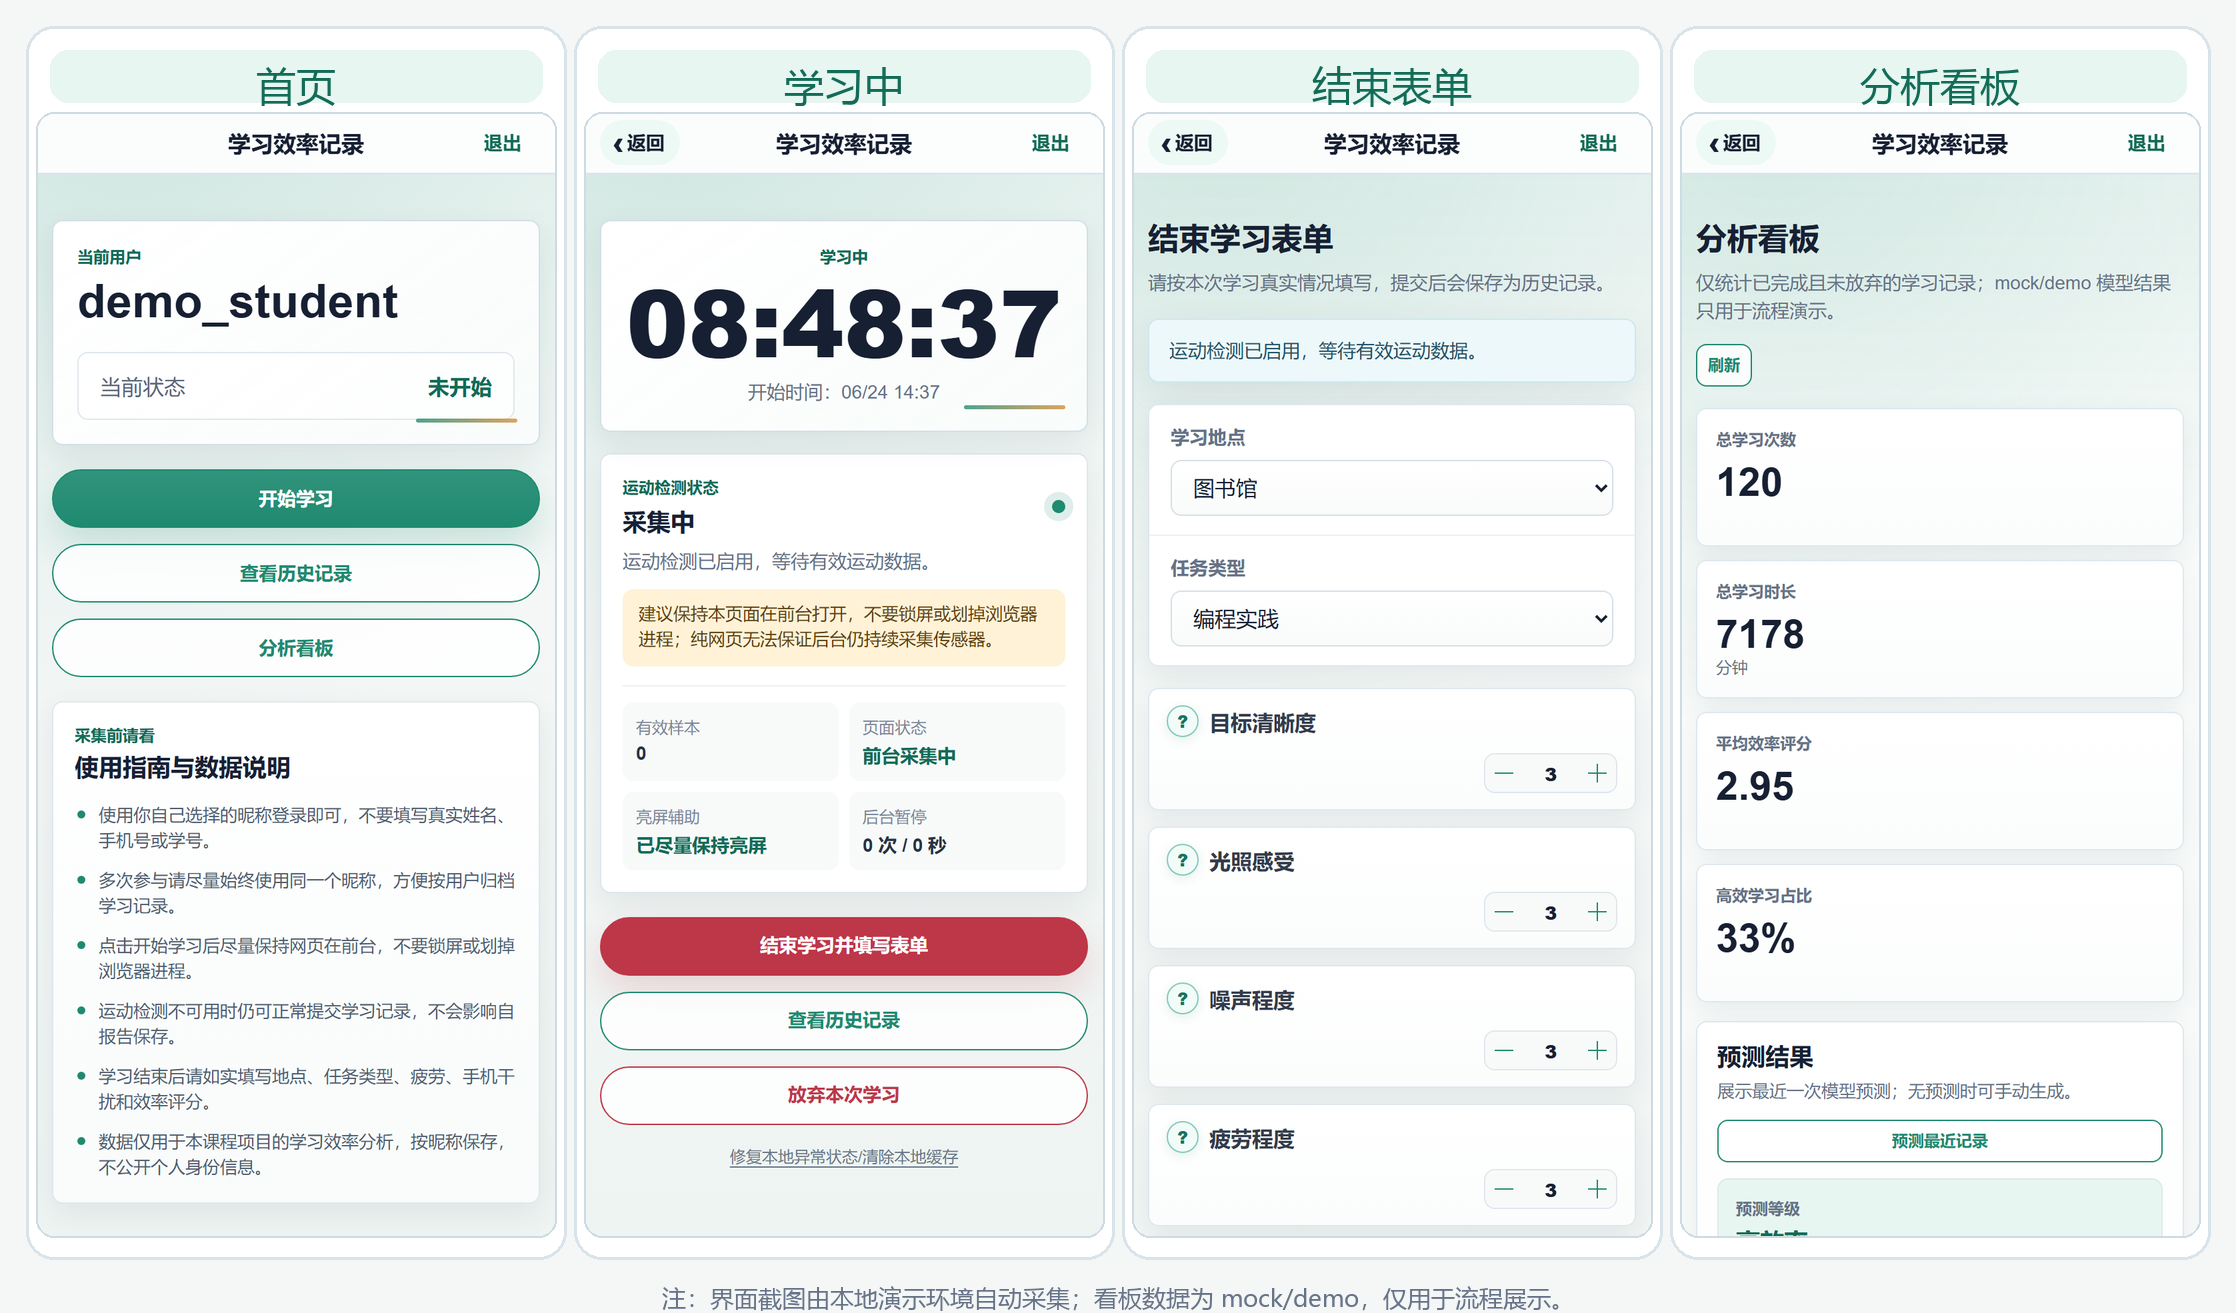
\includegraphics[width=\textwidth]{../figures/fig4-ui-collage.png}
  \caption{手机端主要页面与分析看板真实截图拼图。截图由本地演示环境自动采集；看板数据为 mock/demo 数据，仅用于流程展示。}
  \label{fig:ui}
\end{figure}

\subsection{数据质量与实验口径}

真实数据检查结果显示异常学习时长、自报告越界、枚举值问题和标签转换不一致均为 0，但总样本数未达到 30 条最低训练建议。因此本文采用课程演示口径，避免将 mock 指标包装成真实结论。表 \ref{tab:data} 给出不同数据来源的用途和结论边界。

\begin{table}[htbp]
  \centering
  \caption{数据来源与实验结果口径}
  \label{tab:data}
  \small
  \begin{tabularx}{0.95\textwidth}{p{2.1cm}p{4.0cm}p{3.4cm}X}
    \toprule
    数据类型 & 样本量/分布 & 用途 & 结论边界 \\
    \midrule
    真实数据 & completed=17；low=4、medium=11、high=2；motion 缺失 11 条 & 说明真实采集与质量检查 & 少于 30 条，不形成正式模型有效性结论。 \\
    mock 数据 & 120 条；low/medium/high 各 40 条 & 训练、预测、看板流程演示 & 仅证明系统链路可运行，不代表真实学习规律。 \\
    测试/演示记录 & 开发过程产生 & 接口与页面验证 & 不得计入真实实验结果。 \\
    \bottomrule
  \end{tabularx}
\end{table}

\subsection{模型与看板演示结果}

在 120 条 mock 数据上，随机森林训练、指标读取、特征重要性展示和预测 API 链路均可运行。由于 mock 数据是按规则构造的，Accuracy 和 F1-macro 达到 1.000 只说明流程验证通过，不能证明真实场景中的模型泛化能力。

\begin{figure}[htbp]
  \centering
  \begin{subfigure}[t]{0.47\textwidth}
    \centering
    \begin{tikzpicture}
      \begin{axis}[
        width=\linewidth,
        height=4.8cm,
        ybar,
        ymin=0,
        ymax=1.1,
        bar width=8pt,
        symbolic x coords={Acc,Prec,Recall,F1},
        xtick=data,
        ylabel={指标值},
        legend style={at={(0.5,1.12)},anchor=south,legend columns=2,draw=none},
        nodes near coords,
        nodes near coords style={font=\scriptsize},
        grid=major,
        grid style={black!6}
      ]
        \addplot[fill=journalteal,draw=journalteal] coordinates {(Acc,1.000) (Prec,1.000) (Recall,1.000) (F1,1.000)};
        \addplot[fill=journalorange,draw=journalorange] coordinates {(Acc,0.333) (Prec,0.111) (Recall,0.333) (F1,0.167)};
        \legend{RandomForest, Dummy baseline}
      \end{axis}
    \end{tikzpicture}
    \caption{mock 数据上的流程验证指标}
  \end{subfigure}
  \hfill
  \begin{subfigure}[t]{0.47\textwidth}
    \centering
    \begin{tikzpicture}
      \begin{axis}[
        width=\linewidth,
        height=4.8cm,
        xbar,
        xmin=0,
        xmax=0.17,
        xtick={0,0.05,0.10,0.15},
        xticklabels={0,0.05,0.10,0.15},
        xticklabel style={font=\scriptsize},
        ytick=data,
        yticklabels={noise,phone,mood,light,move},
        xlabel={重要性},
        point meta=x,
        nodes near coords={\pgfmathprintnumber[fixed,precision=3]\pgfplotspointmeta},
        nodes near coords align={horizontal},
        nodes near coords style={font=\scriptsize},
        grid=major,
        grid style={black!6}
      ]
        \addplot[fill=journalteal,draw=journalteal] coordinates {
          (0.151744,0)
          (0.147538,1)
          (0.114447,2)
          (0.113204,3)
          (0.089503,4)
        };
      \end{axis}
    \end{tikzpicture}
    \caption{Top 5 特征重要性}
  \end{subfigure}
  \caption{课程演示模型指标与特征重要性。指标来自 mock 数据，仅用于验证 Python 训练和看板链路。}
  \label{fig:result}
\end{figure}

\section{讨论}

第一，真实样本数不足是当前最大限制。17 条 completed 记录可以证明系统已能真实采集，但不适合划分稳定训练集和测试集。后续至少应补充到 50 条以上，并检查三类标签是否平衡。

第二，手机运动特征存在兼容性限制。Web 页面无法保证锁屏或后台时持续采集传感器数据，且不同手机和浏览器支持程度不同。因此本项目将 \texttt{motion\_features} 设计为可选输入，并在特征工程中显式记录 \texttt{motion\_available}。

第三，\texttt{efficiency\_score} 是主观自评标签，不等同于客观成绩或真实学习成果。模型预测的是“自评学习效率等级”，适合课程实验和个人反思，不应推广为对所有大学生学习效率的普遍判断。

第四，本项目允许使用 AI 工具辅助整理材料，但报告中尽量使用系统截图、流程图和数据表作为主图，避免使用与项目无关的生成式插画，降低明显 AI 痕迹。

\section{总结}

本课程设计完成了一个基于手机轻量感知与自报告数据的大学生学习效率预测系统原型。系统覆盖手机端学习记录、FastAPI 后端存储、训练数据导出、质量检查、随机森林三分类、预测接口和分析看板展示，体现了 Python 后端开发、数据处理、机器学习建模和物联网轻量感知的综合应用。当前版本已经适合课程答辩演示；后续可在增加真实样本、优化传感器采集稳定性、补充模型对比实验和完善部署环境后继续迭代。

\section*{成员与分工}

论文开头成员：\memberone；\membertwo。结尾成员：陈嘉宏、蔡天成。

\begin{table}[H]
  \centering
  \caption*{成员分工表}
  \small
  \begin{tabularx}{\linewidth}{p{2.4cm}Xp{1.4cm}}
    \toprule
    成员 & 主要分工 & 占比 \\
    \midrule
    \memberone & 系统需求分析、后端接口、数据字典、模型训练脚本、论文结果整理 & 50\% \\
    \membertwo & 前端页面、手机运动采集、看板展示、PPT 制作、演示与材料整理 & 50\% \\
    \bottomrule
  \end{tabularx}
\end{table}

\begin{thebibliography}{9}
  \bibitem{python} Python Software Foundation. Python Language Reference.
  \bibitem{fastapi} FastAPI Documentation. FastAPI framework, high performance, easy to learn.
  \bibitem{vue} Vue.js Documentation. The Progressive JavaScript Framework.
  \bibitem{sklearn} Pedregosa, F. et al. Scikit-learn: Machine Learning in Python. \textit{Journal of Machine Learning Research}, 2011.
  \bibitem{rf} Breiman, L. Random Forests. \textit{Machine Learning}, 2001.
  \bibitem{mdn} MDN Web Docs. DeviceMotionEvent.
  \bibitem{sqlalchemy} SQLAlchemy Documentation. The Python SQL Toolkit and Object Relational Mapper.
\end{thebibliography}

\end{document}
